\begin{figure}[bth!]
	\begin{center}
		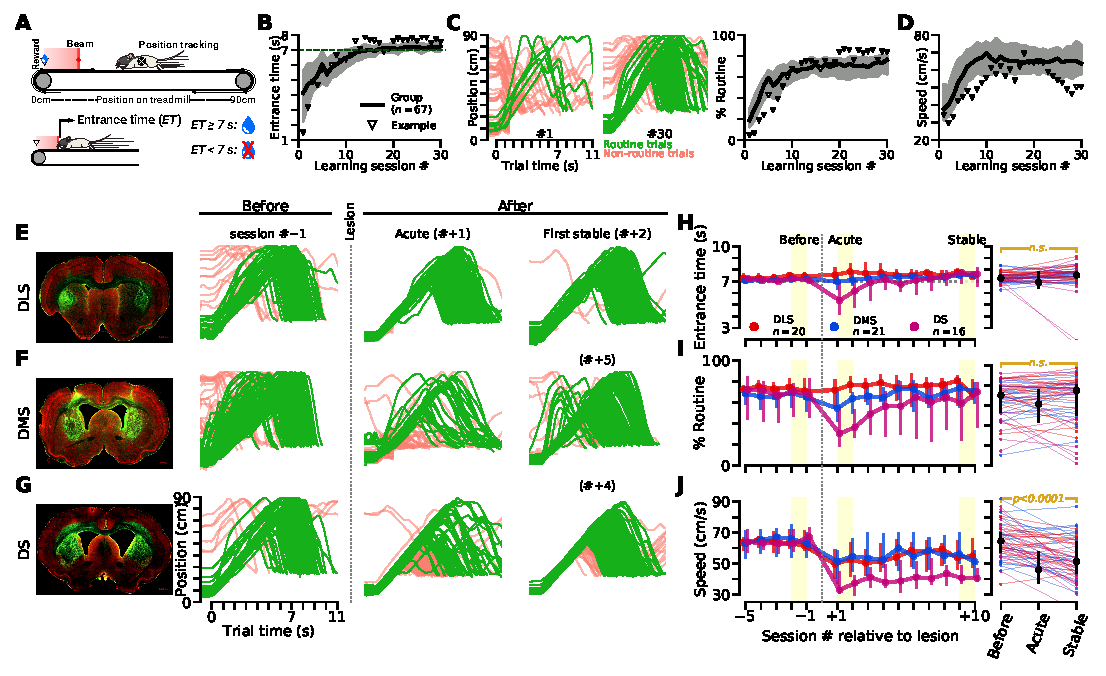
\includegraphics[width=\textwidth]{ch-lesion/figures/Task_Example_Group.pdf}
		\caption
		{\textbf{The dorsal striatum is necessary to invigorate the running component of a motor routine.}
		\textbf{A)} Experimental apparatus and task rules.
		\textbf{B)} Entrance time across training sessions for all the rats trained in this task.  
		Shaded area represents the interquartile range.
		\textbf{C)} Trajectories of an example animal on the treadmill, for all the trials performed during sessions \#1 and \#30 (\textit{left}).
		Percentage of trials during which animals performed the wait-and-run routine, across sessions (\textit{right}).
		\textbf{D)} Running speed when animals ran toward the reward area, across sessions.
		Triangles in panels~B to~D indicate the changes in performance for the example animal whose trajectories are shown in panel~C (\textit{left}).
		\textbf{E-G)} Histology (1st column, GFAP in green shows gliosis, red is NeuN) and trajectories of single animals with bilateral lesions of the dorsolateral, dorsomedial and entire dorsal striatum (\textit{E}: DLS, \textit{F}: DMS, \textit{G}: DS).
		\#~indicates session number relative to the lesion break.
		\textbf{H-J)} \textit{Left}, time course of the lesion effect on ET (\textit{H}), percentage of routine usage (\textit{I}) and running speed (\textit{J}).
		\textit{Right}, group data statistical comparison before vs. after lesion (10000 resamples).
		Trajectories in panels~C,~E,~F and~G are cut after ET.
		}
		\label{fig:lesion:task}
	\end{center}
\end{figure}